\section{MST}

cost/weight function
$w: E \rightarrow \mathbb{N}/\mathbb{R}$

\subsection{Red rule}

$\forall$ cycle colour red the most expensive edge. $\Rightarrow$ the graph without all the red edges is a MST.\\

Search cycle; $m = \#edges, n = \#vertices , m \geq n-1 \Rightarrow  \mathcal{O}(n)$ \\

Selecting max: $\mathcal{O}$(\#vertices in the cycle) = $\mathcal{O}(n)$ \\

How many times do one needs to search in the graph for a cycle: \\ $\mathcal{O}(m-n) = \mathcal{O}(m)$ (until the graph is tree)

$$ \Rightarrow \mathcal{O}(n) \cdot \mathcal{O}(m) = \mathcal{O}(m \cdot n) = \mathcal{O}(n^3)$$

\subsection{Cut-concept}
\begin{center}
	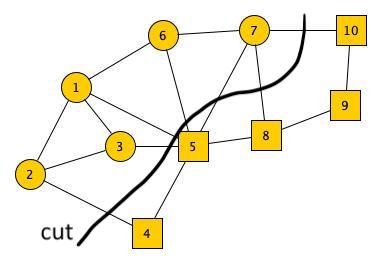
\includegraphics[scale=0.5]{img/graph2}
\end{center}

\begin{itemize}
\item separate the vertices into two sets $V = X \cup X'$, where $X,X'$ are non trivial sets.
\item  all the edges that cut the partition/cross the cut
\item  $\exists$ MST that contains the edge with the minimum weight.
\end{itemize}

\subsection{Blue rule}

$\forall$ cut, colour blue the cheapest edge.

\subsection{Invariant}
$\exists MST(G) T: B \leq T, R \cap T = \emptyset $ \\
$B$ = set of all the blue coloured edges \\
$R$= set of all the red coloured edges

\paragraph{Proof}
base case: $B = \emptyset, R = \emptyset$ holds, because there exists a MST because of all the trees in G, just take the minimum one. Therefore $B \leq T \checkmark, R \cap T = \emptyset \checkmark$ \\

inductive step: \\
RED RULE: edge e \\
in the previous step e is not coloured
\begin{enumerate}
\item edge is not contained in T $\Rightarrow$ Red rule holds
\item edge is contained in T $\Rightarrow$ walk along the cycle and take a edge into T that $w(e') \leq (e)$ $\Rightarrow$ holds
\end{enumerate}

BLUE RULE: edge e \\
was not coloured in the previous step
\begin{enumerate}
	\item e is part of T $\Rightarrow$ Blue rule holds
	\item  e is not part of $T$; $e = (u,v)$, $(u,v)$ were connected with a path and $u \in X$ and $v \in X'$ for every transition along the path $(v' \rightarrow v'') = e'$. $W(e') \geq w(e)$ so it is possible to just take $e$ and leave our $e'$.
\end{enumerate}


\paragraph{COMPLETENESS}
Suppose there is a situation where no rule can be applied to an uncolored edge $e$ \\
blue edges: there is no cycle $\Rightarrow$ blue edges form a forest
\begin{enumerate}
\item  $e$ connects two vertices in the same tree $\Rightarrow$ RED RULE can be applied ($\Rightarrow$ colour it red)
\item $e$ connects two different trees $\Rightarrow$ look at the cut of the two different treefs (B) $\Rightarrow$ BLUE RULE can be applied
\end{enumerate}
There are 7 algorithms that deal with the problem.

\subsection{Kruskal}

Sort the edges in non-decreasing order. Consider the edge next in the order $(u,v)$. \\
if $u$ and $v$ belong to the same subtree $\Rightarrow (u,v)$ red \\
if $u$ and $v$ connect two different subtrees $\Rightarrow (u,v)$ blue

$\mathcal{O}(m \cdot \log m)$